\section{推定 : 信頼区間の読み方と使い方}

  \subsection{問い : SEを, 誰にでも伝わる幅に直す}

    前章で, 平均を取り直したときのばらつきの幅が, 標準誤差 $\mathrm{SE} = s/\sqrt{n}$ という一行の計算で見積もれるようになった.
    報告や記録には平均とあわせてSEを書き添える, というところまでが前章の話だった.

    ただ, 報告を受け取る側の立場で考えると, まだ物足りない.
    「平均はおよそ4.2, SEはおよそ0.1です」と言われて, その平均をどこまで信用してよいのか, すぐに読み取れる人は少ない.
    SEの定義を知っている相手ならともかく, 多くの読み手にとってSEは馴染みのない数字だ.
    せっかく計算したばらつきの目安が, そのままでは相手に届かない.

    届く形は, おそらく幅だ.
    「本当の平均は, だいたい4.0から4.4の間で見ています」と言われれば, 統計を知らない相手でも意味が取れる.
    SEという一つの数字を, こうした幅のかたちに直せないだろうか.

    直すこと自体は, じつは簡単で, SEをおよそ2倍して平均の左右に広げるだけでよい.
    問題はそのあとに待っている.
    作った幅の「だいたい」とは, どのくらいの確かさなのか.
    「この幅の中に本当の平均がある」と言い切ってよいのか.
    ここが, 統計を使う人が最もよく間違えるところであり, 作り方より先に読み方を固めておく必要がある.

    そのうえで, 幅の作り方を平均以外にも広げる.
    章の終わりには, 平均・割合・2群の差のそれぞれについて幅つきで報告でき, その幅が何を意味するかを一文で説明できるようになる.

  \subsection{信頼区間 : 幅の作り方と読み方}

    \subsubsection*{SEから幅へ}

    前章の例をもう一度使う.
    ある商品のレビュー評価は全部で1000件あり, 手元にはそのうち50件だけがある.
    50件の平均は $\bar{x} = 4.2$ だった.
    知りたいのはレビュー全体の平均, つまり母平均 $\mu$ である.

    いちばん素直なのは, 「母平均はおよそ4.2だろう」と, 手元の値をそのまま見積もりに使うことだ.
    このように母数を一つの値で見積もることを\textbf{点推定}と呼ぶ.
    ただ, 前章で見たとおり, $\bar{x}$ は標本を取り直すたびに異なる値をとる.
    つまり, $\bar{x}$ をそのまま $\mu$ だと言い切ってしまうのは, 少し心もとない.

    では, $\bar{x}$ だけを頼りに, $\mu$ の居場所をどこまで絞り込めるだろうか.

    もし $\bar{x}$ が毎回まったく同じ値になるなら, 話は簡単だ.
    その値がそのまま $\mu$ だと言えばいい.
    しかし実際には $\bar{x}$ はばらつく.
    そのばらつきの幅は, 前章で導入した標準誤差 $\mathrm{SE}$ で測れるのだった.
    ばらつきの幅がわかっているなら, 「$\bar{x}$ は $\mu$ からそう遠くないはずだ」ということを, もう少し具体的に言えそうだ.

    ここで, 前章の中心極限定理が効いてくる.
    標本サイズが十分大きければ, $\bar{x}$ はおよそ正規分布に従う.
    正規分布の形がわかっているおかげで, 「$\bar{x}$ が $\mu$ からどのくらい離れうるか」を確率で語れる.
    具体的には, $\bar{x}$ が $\mu$ を中心として $\pm 1.96 \times \mathrm{SE}$ の範囲に収まる確率がおよそ95\%だ.
    1.96という数は, 前章の「$\pm 2\sigma$ に約95\%」の「約」を細かくしたもので, 正規分布では平均から標準偏差の1.96倍以内に全体のちょうど95\%が収まる.
    この関係を $\mu$ の側から書き直すと, 次の区間が得られる.

\begin{defi}{95\%信頼区間}{ci95}
  標本平均を $\bar{x}$, その標準誤差を $\mathrm{SE}$ とするとき,
  \[
    \bar{x} - 1.96 \times \mathrm{SE} \;\leq\; \mu \;\leq\; \bar{x} + 1.96 \times \mathrm{SE}
  \]
  を満たす範囲を, 母平均 $\mu$ の\textbf{95\%信頼区間}と呼ぶ.
\end{defi}

    式の作りを確かめておこう.
    区間の中心は $\bar{x}$ で, そこから左右に $1.96 \times \mathrm{SE}$ ずつ広げている.
    $\mathrm{SE}$ は $\bar{x}$ 自身のばらつきの幅だから, この区間は「$\bar{x}$ が動きうるぶんだけ, $\mu$ の候補に余裕を持たせた範囲」になっている.

    レビューの例で作ってみる.
    50件の標準偏差が $s = 0.7$ だったとすると, $\mathrm{SE} = 0.7/\sqrt{50} \approx 0.10$.
    区間は $4.2 \pm 1.96 \times 0.10$ で, およそ $4.0$ から $4.4$ となる.
    「レビュー全体の平均は4.0から4.4の間で見ている」と, 幅のかたちで言えるようになった.

    実際の計算では, 1.96を「およそ2」に丸めて $\bar{x} \pm 2 \times \mathrm{SE}$ と概算して差し支えない.
    本書でも以降はこの概算を使う.
    なお, 標本が小さいときは, この「2」をもう少し大きめにする必要がある.
    本書では $n$ がそこそこ大きく, 2で足りる場合を扱う.

    \subsubsection*{95\%の正しい読み方}

    さて, 4.0から4.4という区間ができた.
    残る問題は, この「95\%」をどう読むかだ.
    「95\%の確率で $\mu$ がこの区間にいる」と読みたくなるかもしれないが, それは正確ではない.

    $\mu$ は未知ではあるが, 動かない.
    レビュー全体の平均は, 誰にも知られていないだけで, 固定された一つの値だ.
    動くのは $\bar{x}$ のほうであり, したがって区間のほうだ.
    標本を取り直せば $\bar{x}$ は違う値になり, 区間も毎回違う場所にできる.

    このことは, 母平均を知っている立場から眺めるとはっきりする.
    かりにレビュー全体の平均が $\mu = 4.1$ だと分かっている世界を用意して, 50件の標本から $\bar{x} \pm 2 \times \mathrm{SE}$ の区間を作る手順を100回繰り返してみる.
    その結果が\cref{fig:ch05_ci_coverage}だ.

    \begin{figure}[htbp]
      \centering
      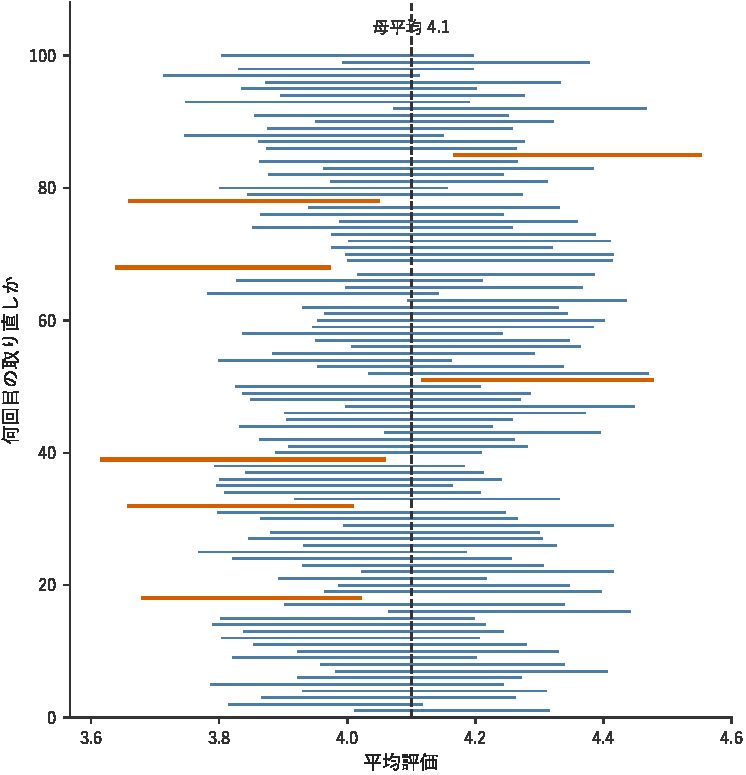
\includegraphics[width=0.8\linewidth]{../figures/output/ch05_ci_coverage.pdf}
      \caption{母平均4.1, 標準偏差0.7の仕組みから50件の標本を取り, 95\%信頼区間を作る手順を100回繰り返したシミュレーション. 横棒の1本1本が1回分の区間. 破線は母平均で, 動かない. 100本のうち93本(細い棒)は母平均を含み, 7本(太い棒)は外した.}
      \label{fig:ch05_ci_coverage}
    \end{figure}

    100本の区間は, どれも少しずつ違う場所にできている.
    そして, そのうち93本は $\mu = 4.1$ を含み, 7本は外した.
    95本ちょうどではないが, 100回の繰り返しをやり直せば, この本数は95前後で毎回すこし変わる.
    95\%とは, 一本一本の区間が持っている性質ではなく, この\textbf{手順の当たりやすさ}のことなのだ.

    では, 手元の一本, 4.0から4.4はどうか.
    図の中から棒を一本選んで「この区間は母平均を含んでいますか」と聞かれたら, 答えは含んでいるか, いないかの二つに一つだ.
    「95\%の確率で含んでいる」という状態は, 図のどこにもない.
    手元の区間も同じで, 当たりか外れかのどちらかであり, どちらなのかは $\mu$ を知らない私たちには分からない.

    それでも, この区間は信用して報告に使ってよい.
    ただし, 信用の根拠は区間そのものにではなく, 区間を作った手順の側にある.
    この手順で区間を作れば, 繰り返したとき95\%は母平均を含むように設計されている.
    手元の一本は, その手順から出てきた一本だ.
    だから95\%信頼区間は, 「この区間に $\mu$ がある確率が95\%」ではなく, 「\textbf{繰り返せば95\%当たる作り方で作った区間が, これだ}」と読む.
    区間を受け取った人も, 同じ読み方をすればよい.
    「100回中95回当たる手順の1回分」という意味合いさえ共有されていれば, 幅の解釈が人によって食い違うことはない.

    \subsubsection*{幅があると何が変わるか}

    読み方が定まったところで, 幅を添えることが実際の判断でどう効くかを見ておこう.

    新薬の治験で「血圧を平均5\,mmHg下げた」という結果が出たとする.
    95\%信頼区間が2〜8\,mmHgなら, 「少なくとも2\,mmHgは下がりそうだ」と見込める.
    医師はこの情報をもとに投薬を判断できる.
    ところが同じ「平均5下がった」でも, 区間が$-1$〜$11$\,mmHgなら話は変わる.
    幅の中にゼロやマイナスが入っている以上, 「効かない可能性も, むしろ上がる可能性も, 取り直しのばらつきの範囲内」ということになり, 判断は慎重にならざるをえない.
    点の値だけを見ていたら, この二つの状況は区別できない.

    幅を添えた報告は, 見積もりの値だけでなく, その見積もりの精度まで相手に渡す.
    過大な断言を防ぎ, 判断ミスを減らすのは, この「精度ごと渡す」働きだ.

    \subsubsection*{何\%にするかは, 人が決める}

    ここまでの手続きのうち, 何が理論から決まっていて, 何が人間の選択なのかを整理しておく.

    「$\bar{x}$ がおよそ正規分布に従う」という部分は, 中心極限定理から導かれる帰結だ.
    ここに人間の裁量は入っていない.
    一方, 「繰り返したとき何\%当たる手順にするか」は, 使う側が決めることだ.
    この割合を\textbf{信頼水準}と呼ぶ.
    信頼水準を決めると, 正規分布の形から, SEの何倍まで広げればよいかが対応して決まる.

    \begin{itemize}
      \item 90\%なら $\pm 1.64 \times \mathrm{SE}$
      \item 95\%なら $\pm 1.96 \times \mathrm{SE}$
      \item 99\%なら $\pm 2.58 \times \mathrm{SE}$
    \end{itemize}

    本書ではこの3行で足りる.

    99\%にすれば外す回数は100回中1回に減るが, そのぶん幅は広がる.
    90\%にすれば幅は狭くなるが, 10回に1回は外す手順になる.
    どのくらいの外れを許容するかは, 分析の目的に応じて選ぶものであり, 理論が一意に決めるものではない.
    95\%が広く使われているのは, 幅の狭さと外しにくさのバランスが実用上とりやすいからで, それ以上の根拠はない. 慣習だ.

  \subsection{やり方 : 3つのケースで幅を作る}

    \subsubsection*{前提}

    以降の計算が仮定するのは, 前章の中心極限定理と同じく, 観測値が独立同分布(i.i.d.)であることの1点である.
    標本サイズの大きさは前提ではなく近似の精度の問題であることも, 前章で整理したとおりだ.

    幅の作り方は, どのケースでも共通している.
    見積もりたい量の推定値を計算し, その推定値のSEを求め, 推定値 $\pm 2 \times \mathrm{SE}$ とする.
    ケースごとに変わるのは, SEの計算式だけだ.

    \subsubsection*{ケース1 : 平均に幅をつける}

    ある商品の重量を $n = 64$ 個測ったところ, 平均 $\bar{x} = 170$\,g, 標準偏差 $s = 12$\,gだった.

    SEは $12/\sqrt{64} = 12/8 = 1.5$\,g.
    95\%信頼区間は
    \[
      170 \pm 2 \times 1.5 \;\Rightarrow\; 167.0\;\text{g〜}\;173.0\;\text{g}.
    \]

    この幅が「広い」か「狭い」かは, 何と比べるかで決まる.
    たとえばこの商品の規格が「165〜175\,gに収まること」なら, 区間はすっぽり規格内に入っており, 安心材料になる.
    規格が「169〜171\,g」と厳しければ, 区間が規格からはみ出しており, $n$ を増やして見積もりの精度を上げるなどの対策が要る.
    幅そのものに良い悪いはなく, 評価は文脈が決める.

    \subsubsection*{ケース2 : 割合に幅をつける}

    20本の作品のうち, 平均評価が4.0以上のものが $k = 14$ 本だったとする.
    標本での割合は $p = 14/20 = 0.70$ だ.
    知りたいのは, 母集団全体でこの割合がいくらか, である.

    割合にも同じ作り方が通用する.
    各作品を「4.0以上なら1, 未満なら0」と数値にしてみると, 割合 $p$ はこの0と1の平均にほかならない.
    平均である以上, 中心極限定理がそのまま効いて, $p$ の取り直しのばらつきもおよそ正規分布に従う.
    そのSEは次の式で見積もれる.
    \[
      \mathrm{SE}(p) \approx \sqrt{\frac{p(1-p)}{n}} = \sqrt{\frac{0.70 \times 0.30}{20}} \approx 0.102.
    \]

    分子の $p(1-p)$ は, 0と1のデータの散らばりの大きさに当たる.
    $p$ が0.5に近いほど0と1が混ざり合って散らばりは大きく, 0や1に近いほど値が片側に揃って小さくなる.
    分母の $n$ は件数で, 多いほどSEは小さくなる.
    平均のSEと同じ構造だ.

    95\%信頼区間は
    \[
      0.70 \pm 2 \times 0.102 \;\Rightarrow\; 0.50\;\text{〜}\;0.90.
    \]

    かなり広い.
    「半分」から「9割」までの範囲では, 見積もりとしてほとんど絞り込めていない.
    $n = 20$ では, 割合の推定はこの程度の精度にとどまる.

    \subsubsection*{ケース3 : 2つの平均の差に幅をつける}

    グループAとBで, 値の平均を比べたいとする.
    見積もりたい量は平均の差 $\bar{x}_A - \bar{x}_B$ だ.
    2群が互いに独立である(AとBで別の個体から集めている)とき, 差のSEは各群の標準偏差 $s_A, s_B$ と件数 $n_A, n_B$ から見積もれる.
    \[
      \mathrm{SE}(\bar{x}_A - \bar{x}_B) \approx \sqrt{\frac{s_A^2}{n_A} + \frac{s_B^2}{n_B}}.
    \]

    根号の中は, それぞれの群の分散を件数で割ったものの和だ.
    $s_A^2/n_A$ は $\bar{x}_A$ の, $s_B^2/n_B$ は $\bar{x}_B$ のばらつき(SEの2乗)であり, 2群が独立なら, 差のばらつきはこの2つの足し算になる.
    引き算をしているのに, ばらつきのほうは差し引かれない.
    もし2群が連動して同じ方向にずれるなら, 差を取った時点でずれどうしが打ち消し合い, ばらつきは小さくなりうる.
    しかし独立なら, $\bar{x}_A$ のずれと $\bar{x}_B$ のずれは無関係に生じるから, 打ち消し合いは期待できず, どちらのずれもそのまま差に持ち込まれる.
    両方の変動が加わるぶん, ばらつきの大きさを表す分散は積み重なる.
    差がどちらか一方の平均だけよりも大きくばらつくのは, その結果だ.

    幅は同じく, 差 $\pm 2 \times \mathrm{SE}$ とする.
    差の区間を読むときは, まずゼロをまたぐかどうかを見る.
    またいでいれば, 「差がない(ゼロ)」も取り直しのばらつきの範囲内にあることになり, 差の向きすら言い切れない.
    またいでいなければ, 少なくとも差の向きは, ばらつきを見込んでも保たれている.

  \subsection{実践 : 80本の映画に幅を添える}

    ランニング例に戻ろう.
    手元にあるのは, 配信サービスの対象作品から抽出された邦画80本の標本だった.
    第1章で置いた「標本は対象作品全体から大きな偏りなく抽出されたものとして扱う」という仮定を, ここでも使う.
    3つのケースを順に当てはめて, 対象作品全体について幅つきで言えることを確かめていく.

    \subsubsection*{平均 : 視聴回数はどのくらいか}

    80本の視聴回数は, 平均 $\bar{x} = 209.4$ 万回, 標準偏差 $s = 239.3$ 万回だった.
    SEは
    \[
      \mathrm{SE} = \frac{239.3}{\sqrt{80}} \approx 26.8\;\text{万回}
    \]
    となり, 95\%信頼区間は
    \[
      209.4 \pm 2 \times 26.8 \;\Rightarrow\; 155.9\;\text{万回〜}\;262.9\;\text{万回}.
    \]

    報告するなら, たとえば次のような一文になる.
    「対象作品の平均視聴回数は209万回と推定される(95\%信頼区間 : 156万〜263万回).」
    信頼水準と幅を添えておけば, 受け手は「繰り返せば95\%当たる作り方での見積もり」として, 精度ごと受け取れる.

    \subsubsection*{割合 : 評価4.0以上の作品はどのくらいあるか}

    80本のうち, 平均評価が4.0以上の作品は33本だった.
    標本での割合は $p = 33/80 \approx 0.41$.
    SEは
    \[
      \mathrm{SE}(p) \approx \sqrt{\frac{0.41 \times 0.59}{80}} \approx 0.055
    \]
    となり, 95\%信頼区間は
    \[
      0.41 \pm 2 \times 0.055 \;\Rightarrow\; 0.30\;\text{〜}\;0.52.
    \]

    「対象作品のうち評価4.0以上は41\%と推定される(95\%信頼区間 : 30\%〜52\%)」となる.
    $n = 80$ あっても, 割合の幅は $\pm 11$ ポイントある.
    ケース2の $n = 20$ よりはずっと絞れているが, たとえば幅を $\pm 3$ ポイントまで詰めるには, 1000件ほどが必要になる.

    \subsubsection*{差 : 原作の有無で視聴回数は違うか}

    80本の映画には, 原作のある作品(既存作品の映画化)とない作品(オリジナル脚本)が混ざっている.
    原作あり37本の平均視聴回数は274.1万回(標準偏差257.1万回), 原作なし43本の平均は153.7万回(標準偏差207.2万回)で, 差は120.4万回だった.

    2群は別々の作品からなり, 独立とみなせる.
    差のSEは
    \[
      \mathrm{SE} \approx \sqrt{\frac{257.1^2}{37} + \frac{207.2^2}{43}} \approx 52.8\;\text{万回}
    \]
    となり, 95\%信頼区間は
    \[
      120.4 \pm 2 \times 52.8 \;\Rightarrow\; 14.8\;\text{万回〜}\;225.9\;\text{万回}.
    \]

    区間はゼロをまたいでいない.
    取り直しのばらつきを見込んでも, 「原作あり群のほうが多い」という向きは保たれている.
    ただし下端の14.8万回は, ゼロのすぐ近くだ.
    そして「15万回差」から「226万回差」までは, 差の大きさとしてほとんど別世界であり, 大きさのほうはまだ絞り込めていない.
    この結果をどこまで信じてよいかは, 章の終わりでもう一度考える.

  \subsection{幅を狭めたいとき}

    区間が広すぎて実用にならないと感じたら, 打てる手は3つある.

    第一に, $n$ \textbf{を増やす}.
    SEは $1/\sqrt{n}$ のペースで縮むから, $n$ を4倍にすれば幅は半分になる.
    「あと何件集めれば幅がどのくらい縮むか」を, この関係から前もって見積もれる.

    件数の効果を具体的に見ておこう.
    平均3.8, $s = 0.9$ のデータで, 件数だけが違う場合を比べる.
    \begin{itemize}
      \item $n = 5$ : $\mathrm{SE} = 0.9/\sqrt{5} \approx 0.40$ で, 幅は $\pm 0.80$
      \item $n = 20$ : $\mathrm{SE} = 0.9/\sqrt{20} \approx 0.20$ で, 幅は $\pm 0.40$
      \item $n = 100$ : $\mathrm{SE} = 0.9/\sqrt{100} = 0.09$ で, 幅は $\pm 0.18$
    \end{itemize}
    平均はどれも同じ3.8だ.
    しかし $n = 5$ の幅と $n = 100$ の幅は4倍以上違う.
    「平均が同じなら同じことを言っている」わけではない.
    レビューサイトで星4.2の店が2軒あっても, 件数5件の4.2と件数500件の4.2では, 見積もりとしての確かさがまるで違う.

    第二に, \textbf{ばらつき} $s$ \textbf{を下げる}.
    測定条件を安定させる, 対象を絞る, 性質の近い層に分けてから推定する, といった工夫で $s$ が小さくなれば, SEも縮む.

    第三に, \textbf{信頼水準を下げる}.
    95\%を90\%にすれば幅は狭くなる.
    ただし10回に1回外す手順になるので, 幅の狭さを外れやすさで買っていることになる.

    実務でまず検討するのは最初の2つだ.
    信頼水準の変更は見かけの幅を変えるだけで, 見積もりの精度そのものは何も変わっていない.

  \subsection{実務で気をつけること}

    \subsubsection*{偏りは$n$で解決しない}

    ここまでの話には, 見落とすと危険な前提が一つ埋まっている.
    「繰り返せば95\%当たる」という設計が成り立つのは, 手順の入り口, つまり標本の集め方がi.i.d.に近い場合だけだ.
    集め方が偏っていれば, $\bar{x}$ は取り直すたびに, 母平均からずれた場所を中心にばらつく.
    その状態で $n$ を増やすと, 区間は狭くなるのに, 区間の中心は的外れのままという結果になる.
    \textbf{精密に間違える}という, 最も危険な状態だ.
    区間の信用が手順の側にある以上, 手順が壊れていれば, どれほど狭い区間にも信用は残らない.
    区間の狭さに安心する前に, データの集め方をまず点検する.

    \begin{mybox}{ギャラップ vs.\ Literary Digest : 240万人が大はずれした話}
    1936年のアメリカ大統領選挙で, 雑誌 \textit{Literary Digest} は大規模な郵送調査を行った.
    返送されたのは約240万通.
    これだけの数があれば確実に思えるが, 予測は「ランドンの勝利」.
    結果はルーズベルトの圧勝で, 大はずれだった.

    原因は集め方にある.
    \textit{Literary Digest} は電話帳や自動車登録簿から名簿を作ったが, 1930年代にこれらを持っていたのは富裕層に偏っていた.
    さらに, 郵送に返事をする人としない人の間にも偏りがある.
    結果として, 240万人のデータは母集団を代表していなかった.

    一方, ジョージ・ギャラップはわずか約5万人の調査で正しくルーズベルトの勝利を予測した.
    ギャラップは年齢・性別・地域などの構成比を考慮して回答者を集める工夫をしていた.

    \textbf{$n = 240$万でも, 偏りがあれば自信満々に間違える}.
    この事件の後, \textit{Literary Digest} は廃刊に追い込まれた.
    \end{mybox}

    偏りの類型と対処は, 9章で改めて整理する.

    \subsubsection*{外れ値と歪みへの対処}

    平均とSDは外れ値に引っ張られやすい.
    3章でヒストグラムや箱ひげ図から外れ値に気づく方法を扱ったが, ここでの問題は, 外れ値が $\bar{x}$ と $s$ を通じて区間の位置と幅に直接響くことだ.
    きつい外れ値がある場合は, 中央値やIQRで要約し, 幅の作り方も\textbf{ブートストラップ}と呼ばれる別の方法に切り替えるほうが安全なことがある.
    ここでは名前だけの紹介にとどめる.

    データが右に強く歪んでいる場合は, 対数を取ってから扱うとよい.
    前章のコラムで見たとおり, 掛け算の仕組みから生まれた右裾の長い分布は, 対数を取ると足し算の世界に戻り, 釣鐘型に近づく.
    歪みが軽くなるぶん, 同じ $n$ でも正規近似の精度が上がる.
    対数のスケールで平均とSEを計算して幅を作り, 報告のときに必要なら元のスケールに戻す(戻した値は幾何平均に対応する).

    \subsubsection*{前処理の記録}

    推定の幅は, 期間の切り取り方, 欠損値の扱い, 外れ値の処理によって変わる.
    同じデータでも, 前処理が違えば違う区間ができる.
    「何を, いつ, どう集めて, どう処理したか」を明示しておくことが, 結果を他者と共有するための最低限の作法だ.

  \subsection{結果と次の一手 : 幅の先にある問い}

    前章の終わりに, SEを誰が読んでも同じ意味になる幅に直したい, という宿題を立てた.
    本章でその直し方が決まった.
    推定値 $\pm$ 約 $2 \times \mathrm{SE}$ で95\%信頼区間を作り, 平均・割合・差のどれにも同じ作り方を通せる.

    そして, 幅の読み方も決まった.
    95\%は区間そのものの性質ではなく, 区間を作る手順の当たりやすさだ.
    手元の一本が当たりか外れかは分からないが, 繰り返せば95\%当たる作り方で作った一本として報告し, 受け取る.
    この読み方さえ共有されていれば, 幅を添えた報告は, 見積もりの精度ごと相手に渡る.

    新聞の世論調査で「支持率45\%($\pm 3$ポイント)」という表記を見たことがあるかもしれない.
    あの $\pm 3$ ポイントは, まさにここで作った幅と同じものだ.
    次に見かけたら, 「繰り返せば95\%当たる手順の1回分」という意味合いまで読み取れるはずだ.

    最後に, 実践で残した宿題に戻る.
    原作あり群と原作なし群の平均視聴回数の差は, 95\%信頼区間で14.8万〜225.9万回だった.
    区間はゼロをまたがなかったが, 下端はゼロのすぐ近くにある.
    もし標本を取り直していたら, ゼロをまたぐ区間が出ていてもおかしくない.
    そうなると, 「原作あり群のほうが本当に多いのか, それとも, たまたま視聴回数の多い作品が原作あり側に集まっただけなのか」という疑いには, まだ決着がついていない.
    この「差は偶然のばらつきで説明できるか」という問いに正面から答えるには, 幅をつけるのとは別の枠組みが要る.
    それが, 次章で扱う\textbf{統計的検定}だ.

  \begin{mybox}{コラム : 標本平均は信用してよい見積もりか}
    本章では $\bar{x}$ のばらつきに幅をつけてきたが, そもそも $\bar{x}$ で $\mu$ を狙うこと自体は適切なのか, という一段手前の問いもある.
    母数の見積もりに使う統計量を\textbf{推定量}と呼び, その良し悪しを測る性質が知られている.

    一つは, 狙いが系統的にずれていないかだ.
    中心極限定理で見たとおり, $\bar{x}$ の標本分布の中心は母平均 $\mu$ そのものだった.
    取り直しを繰り返したときの $\bar{x}$ の平均が $\mu$ に一致する, つまり高めにも低めにも偏らない.
    この性質を\textbf{不偏性}といい, 標本平均は母平均の不偏推定量である.

    不偏でない例は, じつは第2章にすでに登場している.
    分散を $1/n$ で計算すると, 母集団の分散よりも系統的に小さめの値が出る.
    偏差を母平均 $\mu$ からではなく標本平均 $\bar{x}$ から測っているためだ.
    $\bar{x}$ は手元のデータに最も寄り添う位置に来る値なので, $\bar{x}$ からの偏差の2乗和は, $\mu$ からのそれより必ず小さめになる.
    その縮みぶんを補正したのが, $n$ の代わりに $n-1$ で割る\textbf{不偏分散}だ.
    第2章の脚注で触れた「$n-1$ で割る流儀」の正体は, この補正である.

    もう一つは, 件数を増やせば母数に近づいていくかだ.
    $\bar{x}$ のSEは $s/\sqrt{n}$ だから, $n$ を増やせば $\bar{x}$ の散らばりはいくらでも小さくなり, $\mu$ のまわりに絞り込まれていく.
    この性質を\textbf{一致性}と呼ぶ.

    狙いが系統的にずれず(不偏性), 数を増やせば絞り込める(一致性).
    統計学が標本平均を安心して使うのは, こうした性質の裏づけがあってのことだ.
    実務でここまで確かめる場面は少ないが, 推定量への信用がどこから来ているのかは, 知っておいて損はない.
  \end{mybox}
